%%%%%%%%%%%%%%%%%%%%%%%%%%%%%%%%%%%%%%%%%%%%%%%%%%%%%%%%%%%%%%%%%%%
\documentclass[10pt,landscape]{article}
\usepackage{amssymb,amsmath,amsthm,amsfonts}
\usepackage{multicol,multirow}
\DeclareMathOperator*{\argmax}{arg\,max}
\DeclareMathOperator*{\argmin}{arg\,min}
\usepackage{calc}
\usepackage{tikz}
\usepackage{ifthen}
\usepackage{textcomp}
\usepackage{xcolor}
\usepackage{graphicx}
\usepackage{makecell}
\graphicspath{ {./images/} }
\usepackage{enumitem}
\usepackage{bm}
\usepackage{titlesec}
\usepackage[landscape]{geometry}
\usepackage{fancyhdr}
\usepackage[colorlinks=true,citecolor=blue,linkcolor=blue]{hyperref}
%------------------------------------
\ifthenelse{\lengthtest { \paperwidth = 11in}}
    { \geometry{top=.4in,left=.5in,right=.5in,bottom=.4in} }
	{\ifthenelse{ \lengthtest{ \paperwidth = 297mm}}
		{\geometry{top=1cm,left=1cm,right=1cm,bottom=1cm} }
		{\geometry{top=1cm,left=1cm,right=1cm,bottom=1cm} }
	}
\pagestyle{fancy}
\fancyhf{}
% Remove line
\renewcommand{\headrulewidth}{0pt}
\cfoot{\fontsize{9pt}{11pt}\selectfont Frank Facundo}
\setlength{\footskip}{16pt} % amount to move footer by
% Remember to call your parents and tell them you love them!

% Define smaller plus sign
\newcommand{\plus}{\raisebox{.3\height}{\scalebox{.7}{+}}}

\makeatletter
\renewcommand{\section}{\@startsection{section}{1}{0mm}%
                                {-1ex plus -.5ex minus -.2ex}%
                                {0.5ex plus .2ex}%x
                                {\normalfont\large\bfseries}}
\renewcommand{\subsection}{\@startsection{subsection}{2}{0mm}%
                                {-1ex plus -.5ex minus -.2ex}%
                                {0.5ex plus .2ex}%
                                {\normalfont\normalsize\bfseries}}
\renewcommand{\subsubsection}{\@startsection{subsubsection}{3}{0mm}%
                                {-1ex plus -.5ex minus -.2ex}%
                                {1ex plus .2ex}%
                                {\normalfont\small\bfseries}}
\makeatother
\setcounter{secnumdepth}{0}
\setlength{\parindent}{0pt}
\setlength{\parskip}{0pt plus 0.5ex}
% ----------------------------------------------------

\title{Concurrent systems}
\begin{document}

\raggedright
\footnotesize

\begin{center}
    \vspace{-50mm}
    \Large{\vspace{-15mm}\textbf{Concurrent systems}} \\
    \footnotesize{Last Updated \today}
    \vspace{-.4mm}
\end{center}
\begin{multicols}{3}
    \setlength{\premulticols}{1pt}
    \setlength{\postmulticols}{1pt}
    \setlength{\multicolsep}{1pt}
    \setlength{\columnsep}{2pt}
    % --------------------------------------------------------------
    \section{Concepts}
    \textbf{Liveness} - The operation eventually returns something.
    
    \textbf{Safety} - The operation never returns anything incorrect (an ad-hoc rule).
    
    \textbf{Correct} - Safety and Liveness
    \begin{itemize}[label={--},leftmargin=4mm]
        \vspace{-1mm}
        \itemsep -.4mm
        \item In out context: A process that never \textbf{fails} (stops taking steps) in the middle of middle of its operation is called \textbf{correct}. We tipically assume that a correct process invokes infinitely many operations, so a process is correct if it takes infinitely many steps.

    \end{itemize}
    \textbf{Progress} - Non blocked, process completes operations in a finite amount of time.

    \subsection{Liveness Properties}
    \textbf{Deadlock-free (DF)} - If every process is correct, some process makes progress.

    \textbf{Starvation-free (SF)} - If every process is correct, every process makes progress.

    \textbf{Lock-free / non-blocking (LF)} - Some correct process makes progress (in a finite number of steps).

    \textbf{Wait-free (WF)} - Every correct process makes progress (in a finite number of steps).

    \textbf{Obstruction-free (OF)} - Every process makes progress if it executes in isolation from some point (it is the only correct process).

    \subsection{Periodic table of liveness properties}

    \begin{center}
        \footnotesize
        \begin{tabular}{ |c|c|c|c| }
            \hline
             & \thead{Independent \\ non-blocking \\ (finite steps)}  &  \thead{Dependent \\ non-blocking}  &  \thead{Dependent \\ blocking \\(infinite steps)} \\
            \hline
            \thead{every          \\process  \\makes \\progress} & wait-freedom                         & \thead{obstruction- \\freedom}      & \thead{starvation- \\freedom} \\
            \thead{some           \\process   \\makes \\progress} & lock-freedom                         & ?                                   & \thead{deadlock- \\freedom}\\
            \hline
        \end{tabular}
    \end{center}
    \textbf{Independent}: Independent of concurrency.

    \textbf{Non-blocking}: At least one proccess make progress.

    \textbf{Independent non-blocking}: Even in concurrency, at least one proccess make progress.

    \textbf{Dependent non-blocking}: When there is no concurrency, at least one proccess make progress.

    \textbf{Dependent blocking}: When there is no concurrency, it is not guaranteed that at least one proccess make progress.



    \subsection{Relations between liveness properties}
    \smallskip
    \begin{center}
        \vspace{-1mm}
        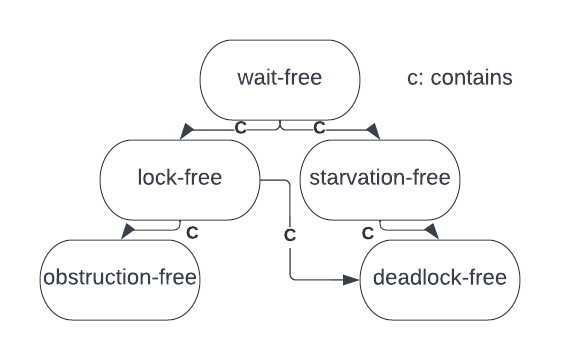
\includegraphics[scale = .8]{images/liveness_properties.png}
    \end{center}
    \vspace{-2mm}

    \section{Register}
    \subsection{Dimensions}
    \begin{itemize}[label={--},leftmargin=4mm]
        \vspace{-1mm}
        \itemsep -.4mm
        \item Value ranges: The set of values that can be stored in the register.
        \item Access pattern: The number of processes that can read or write the register.
              \subitem - single reader: 1R
              \subitem - multi reader: MR
              \subitem - single writer: 1W
              \subitem - multi writer: MW
        \item Concurrent behavior: The correctness guarantees ensured when the register is accessed concurrently.
              \subitem - Atomicity: linearizable
              \subitem - Safety: (single writer) If write does not overlap, return last written value, otherwise return any value in its range.
              \subitem - Regularity: (single writer) If write does not overlap, return last written value, otherwise return value written or the precedent.

    \end{itemize}

    \section{Python}

    \subsection{Library: threading}
    Objects: 
    \begin{itemize}[label={--},leftmargin=4mm]
        \vspace{-1mm}
        \itemsep -.4mm
        \item Thread: Methods: start(), run(), join() \# join wait a thread to be finished to continue. 
        \item Lock: Methods: acquire() [block if already acquired], release(), locked()
        \item RLock: Rentrant lock, recurtion over the same thread.
        \item Condition: Inherits from Lock. Work as synchronized in Java. Methods: acquire(), release(), wait(), notify(), notify\_all()
        \item Semaphore: Inherits from Condition. Classic Dijkstra semaphore. Methods: acquire(), release()
        \item Event: Inherits from Condition. Communication mechanism for threads. Methods: is\_set(), set(), clear(), wait()
        \item Timer: t = Timer(30.0, print\_hello); t.start() \# After 30 seconds hello will be printed.
        \item Barrier: b = Barrier(n) \# b.wait will be blocked until n instances are waiting.

    \end{itemize}

    Which one use? check \href{https://www.laurentluce.com/posts/python-threads-synchronization-locks-rlocks-semaphores-conditions-events-and-queues/}{this link}

    \subsection{Library: syncio}
\end{multicols}

\end{document}